\documentclass[10pt]{scrartcl}

\usepackage[utf8]{inputenc}
\usepackage{tabularx}
\usepackage{longtable}
\usepackage[ngerman]{babel}
\usepackage[automark]{scrpage2}
\usepackage{amsmath,amssymb,amstext}
%\usepackage{mathtools}
\usepackage[]{color}
\usepackage[]{enumerate}
\usepackage{graphicx}
\usepackage{lastpage}
\usepackage[perpage,para,symbol*]{footmisc}
\usepackage{listings} 

\usepackage[numbers,square]{natbib}
\usepackage{color}
\usepackage{colortbl}
\usepackage[absolute]{textpos}
\usepackage{float}
\usepackage{verbatim}
\usepackage[colorinlistoftodos,textsize=small,textwidth=2cm,shadow,bordercolor=black,backgroundcolor={red!100!green!33},linecolor=black]{todonotes}

\usepackage[pdfborder={0 0 0},colorlinks=false]{hyperref}
\usepackage[all]{hypcap}


\lstset{numbers=left, numberstyle=\tiny, numbersep=5pt, breaklines=true, showstringspaces=false} 
\restylefloat{figure}

%changehere
\def\titletext{Lab 2: SIP, Multicast}
\def\titletextshort{Praktikum 2}
\author{André Harms, Oliver Steenbuck}

\title{\titletext}

%changehere Datum der Übung
\date{04.01.2012}

\pagestyle{scrheadings}
%changehere
\ihead{TT1, Schmidt}
\ifoot{Generiert am:\\ \today}

\cfoot{Oliver Steenbuck, André Harms}


\ohead[]{\titletextshort}
\ofoot[]{{\thepage} / \pageref{LastPage}}

\setlength{\parindent}{0.0in}
\setlength{\parskip}{0.1in}

\begin{document}
\maketitle

\setcounter{tocdepth}{3}
\tableofcontents

%	\listoftables                                 												% 
	\listoffigures   

\section{Durchführung des Versuchs}

\subsection{Versuchsaufbau}\label{subsec:versuchsaufbau}
Der Versuch wurde mit der Gruppe Noetzel/Steudte zusammen durchgeführt.
Es wurde pro Gruppe auf einem Rechner der Client gestartet, ein Server wurde nur auf dem Rechner der Gruppe Harms/Steenbuck gestartet. Die IP Adressen der am Versuch beteiligten entsprechenden Rechner waren:
\begin{description}
	\item[Noetzel/Steudte] \verb!141.22.27.34!
	\item[Harms/Steenbuck] \verb!141.22.27.35!
	\item[SIP Gateway] \verb!141.22.27.3!
\end{description}

\subsection{Versuchsplanung} \label{subsec:versuchplanung}
Der Versuch sollte sowohl die SIP Funktionalität der jeweiligen Implementierungen als auch das IGMP Netzwerk im Labor testen. Um diese Ziele zu erreichen wurde folgendes Vorgehen (aus Sicht Server: Steenbuck/Harms) gewählt:

\begin{enumerate}
	\item \verb!Register! beim Proxy
	\item \verb!Invite! durch Client Noetzel/Steudte
	\item \verb!Invite! durch Client Steenbuck/Harms
	\item \verb!Bye! durch Client Noetzel/Steudte
	\item \verb!Bye! durch Steenbuck/Harms
	\item Server Stop
\end{enumerate}

Während des gesamten Versuchablaufes wurde der Netzwerkverkehr aufgezeichnet um diesen später auszuwerten, siehe \ref{sec:beobachtung}.

\subsection{Definition/Darstellung Systemzustände}\label{subsec:systemzusatende}
Aufgrund der Aufgabenspezifikation und der dem Versuch vorhergehenden Tests während der Implementierung haben wir die folgenden Zustände für die am Test beteiligten Komponenten (Server, Clients) definiert:


\subsubsection{Server}
	\begin{description}
		\item[UDPSending] der Server versendet UDP Nachrichten
		\item[UDPWaiting] der Server hat keine aktiven Clients, er versendet keine UDP Nachrichten
		\item[CallWaiting] der Client hat keinen aktiven Call
		\item[CallActive] der Client hat einen aktiven Call
		\item[Registered] der Server ist am Proxy angemeldet
		\item[Shutdown] der Server ist heruntergefahren
	\end{description}
	
\subsubsection{Client}	
	\begin{description}
		\item[CallWaiting] der Client hat keinen aktiven Call
		\item[CallActive] der Client hat einen aktiven Call
		\item[UDPNotReceiving] der Client erhält keine UDP Pakete
		\item[UDPReceiving] der Client erhält UDP Pakete
	\end{description}	
	

	

\subsubsection{Beispiel}

TODO: ??? verstehe nicht, was Du sagen willst
Um darzustellen, dass wir beim Server nach dem der 2. - in \ref{subsec:versuchplanung} beschriebene - Vorgang ausgeführt wurde (\verb!Invite! durch Client Noetzel/Steudte) erwarten, dass der Server am Proxy registriert ist, UDP Nachrichten sendet und einen aktiven call hat nutzen wir folgende Darstellung:

Server:
\begin{enumerate}
	\item --
	\item UDPSending, CallActive, Registered
	\item --
	\item --
	\item --
	\item --
\end{enumerate}

\subsection{Erwartetes Verhalten der Komponenten}\label{subsec:erwartetesSystemverhalten}
Im folgenden ist das erwartete Systemverhalten für Server und beide Clients in der in \ref{subsec:systemzusatende} beschrieben Form dargestellt.

\subsubsection{Server}
\begin{enumerate}
	\item UDPWaiting, CallWaiting, Registered
	\item UDPSending, CallActive, Registered
	\item UDPSending, CallActive, Registered
	\item UDPSending, CallActive, Registered
	\item UDPWaiting, CallWaiting, Registered
	\item Shutdown
\end{enumerate}

\subsubsection{Client Noetzel/Steudte}
\begin{enumerate}
	\item CallWaiting, UDPNotReceiving
	\item CallActive, UDPReceiving
	\item CallActive, UDPReceiving
	\item CallWaiting, UDPNotReceiving
	\item CallWaiting, UDPNotReceiving
	\item CallWaiting, UDPNotReceiving
\end{enumerate}

\subsubsection{Client Harms/Steenbuck}
\begin{enumerate}
	\item CallWaiting, UDPNotReceiving
	\item CallWaiting, UDPNotReceiving
	\item CallActive, UDPReceiving
	\item CallActive, UDPReceiving
	\item CallWaiting, UDPNotReceiving
	\item CallWaiting, UDPNotReceiving
\end{enumerate}

	
	
\section{Beobachtungungen aus dem Versuch} \label{sec:beobachtung}
Mit der unter \ref{subsec:besonderheiten} beschriebenen Ausnahme, zeigten alle Komponenten das unter \ref{subsec:erwartetesSystemverhalten} beschriebene Verhalten.

\subsection{SIP}
	\subsubsection{Register} 
	Der Register SIP Call des Servers (siehe Abbildung: \ref{img:registerServer}) hat dazu geführt, dass korrekt ein Eintrag auf dem Proxy angelegt wurde, dies konnte über die Weboberfläche erfolgreich verifiziert werden.
	
	\begin{figure}[htb]
        \centering
         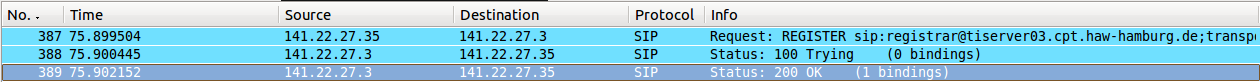
\includegraphics[width=\textwidth]{img/register}
         \caption{Register call des Servers}
        \label{img:registerServer}
	\end{figure}	
	
	\subsubsection{Invite}
	Die Invites der Clients wurden vom Server erfolgreich verarbeitet und bearbeitet. In Abbildung \ref{img:invites} ist der Invite, den der Client Noetzel/Steudte abgesetzt hat, abgebildet. Hier ist auch gut zu erkennen, dass die Kommunikation über den Proxy läuft.

	\begin{figure}[htb]
        \centering
         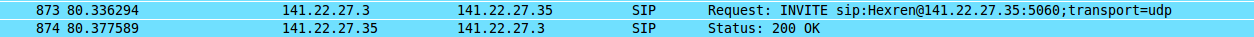
\includegraphics[width=\textwidth]{img/invite}
         \caption{Invite call des Clients Noetzel/Steudte}
        \label{img:invites}
	\end{figure}		

	\subsubsection{Bye}
	Die Byes  der Clients wurden ebenfalls erfolgreich über den Proxy gesendet und vom Server verarbeitet. In Abbildung \ref{img:byes} ist die Abmeldung des Clients Noetzel/Steudte gezeigt.
	
	\begin{figure}[htb]
        \centering
         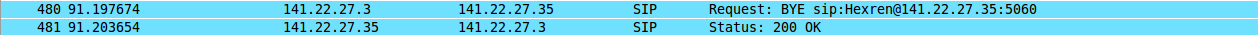
\includegraphics[width=\textwidth]{img/bye}
         \caption{Bye Call des Clients Noetzel/Steudte}
        \label{img:byes}
	\end{figure}		
	

\subsection{IGMP}

	\subsubsection{Join}
	Nach dem invite setzten die Clients erwartungsgemäß IGMP Joins ab, um der Multicastgruppe \verb!239.238.237.17! beizutreten. Die doppelten Join-Nachrichten sind automatisiert durch die Java Multicast Implementierung abgestezt, um UDP Paketverlusten vorzubeugen.
	
	\begin{figure}[htb]
        \centering
         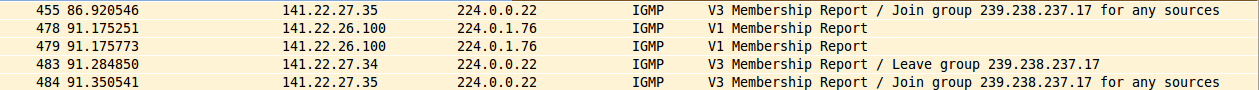
\includegraphics[width=\textwidth]{img/join}
         \caption{IGMP Join des Clients Harms/Steenbuck 141.22.27.35}
        \label{img:join}
	\end{figure}	

	
	\subsubsection{Message Pakete}
	Nachdem der Multicastgruppe	beigetreten wurde, hat die Client Implementierung erfolgreich Nachrichten empfangen. 
	
	\begin{figure}[htb]
        \centering
         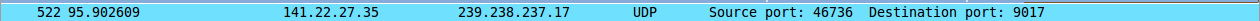
\includegraphics[width=\textwidth]{img/udpMessage}
         \caption{Über Multicast versendete UDP Nachrichten}
        \label{img:udpMessage}
	\end{figure}	
	
	\subsubsection{Leave}
	Nachdem der Call beendet wurde, ist der Client aus der Multicastgruppe ausgetreten. Es sind jedoch weiterhin Nachrichten eingetroffen, siehe \ref{subsec:besonderheiten}.
	
	
	\subsection{Besonderheiten}\label{subsec:besonderheiten}
	
	Die Ergebnisse auf der IGMP Seite der Anwendung entsprechen den Erwartungen (\verb!join! nach \verb!invite! und \verb!leave! nach \verb!bye! auf Clientseite sowie analog auf der Serverseite das starten/stopen des sendens)
	
	Die einzige Ausnahme ist das nach dem clientseitigen \verb!leave! festgestellt wurde, dass wie weiterhin \verb!UDP Multicast! Nachrichten empfangen wurden, siehe Abbildung \ref{img:cap1}. 
	Die Erklärung hierfür dürfte sein, dass die Infrastrutkur in den Laborräumen kein IGMP Snooping unterstützt und daher die Multicastnachrichten über Ethernet Broadcasts implementiert. Diese kommen dann auch bei dem nicht in der Gruppe registriertem Rechner an.
	
	
	\begin{figure}[htb]
        \centering
         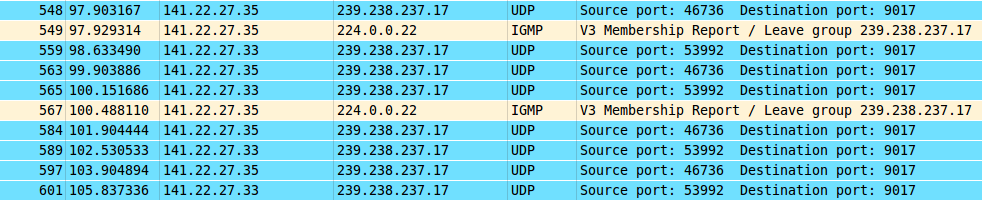
\includegraphics[width=\textwidth]{img/udp_after_leaving}
         \caption{Empfang von UDP Nachrichten nach Austritt aus Multicastgruppe}
        \label{img:cap1}
	\end{figure}	



\section{Anwendung}

\subsection{Starten}
\begin{enumerate}
	\item entpacken \verb!harmsSteenbuckSIP.tgz!
	\item wechseln in das Verzeichnis \verb!dist!
	\item \verb!java -jar "SIPGUI.jar"!
	\item Die unter \ref{sec:bedienung:anwendung} beschrieben Anwendung startet
\end{enumerate}


\subsection{Bedienung}
\label{sec:bedienung:anwendung}		
	\begin{figure}[H]
        \centering
                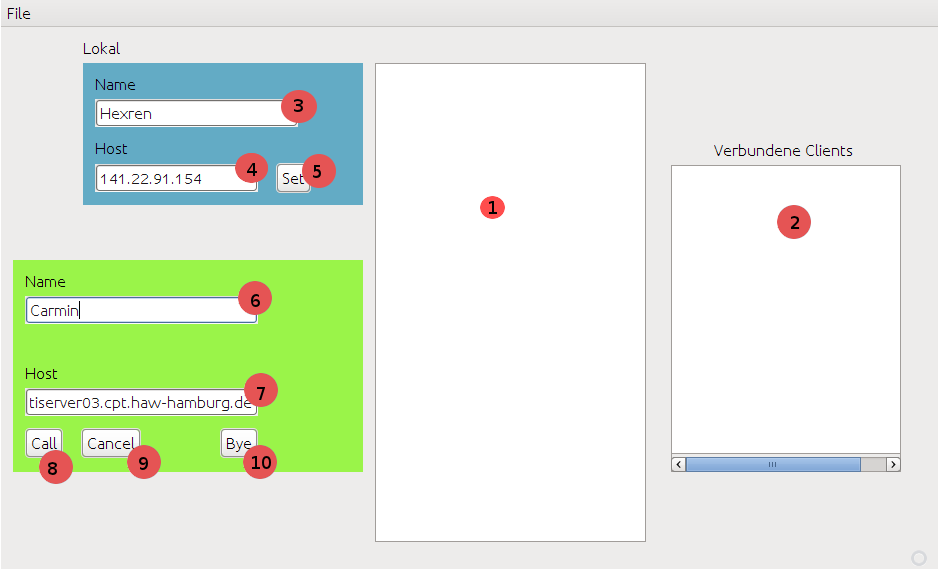
\includegraphics[width=\textwidth]{img/screenshotApplication}
        \caption{Screenshot der GUI}
        \label{img:gui}
	\end{figure}

\begin{enumerate}
	\item Bereich in dem die empfangenen IGMP Nachrichten angezeigt werden
	\item Zum Server verbundene Clients
	\item Name mit dem sich beim Proxy registriert wird
	\item IP Adresse des Rechners
	\item Knopf zum Registrieren
	\item Name des zu invitenden Teilnehmers
	\item IP Adresse des zu invitenden Teilnehmers
	\item Knopf zum Anrufen (inviten) des in X angegebenen Teilnehmers
	\item Knopf zum Abbrechen eines Invites
	\item Knopf zum Beenden der Verbindung
\end{enumerate}

\subsection{Sourcen}
Das Project besteht im wesentlichen aus 2 Teilen. Zum ersten eine Bibliothek, die SIP und IGMP Funktionalitäten bietet und in Eclipse mit Maven entwickelt wurde. Zum anderen eine Oberfläche, die in Netbeans entwickelt wurde und die Bibliothek nutzt. In den Sourcen sollte sich seit der Abgabe nichts mehr geändert haben, im Zweifelsfall ist der commit \verb!fd4d802c26! der letzte vor der Abgabe gewesen.

Die Sourcen für beide Projekte sind auf GitHub unter folgenden Pfaden verfügbar:
\begin{description}
	\item[Bibliothek] Eclipse \\ \verb!https://github.com/MyersGer/WS_2011/tree/master/TT1/Prak2/lab3!
	\item[Oberfläche] Netbeans \\ \verb!https://github.com/MyersGer/WS_2011/tree/master/TT1/Prak2/guiHarmsSteenbuck!
\end{description}

\section{Anlagen}
\begin{itemize}
	\item ausführbare Jar
\end{itemize}

\end{document}

